% $Header: /cvsroot/latex-beamer/latex-beamer/solutions/conference-talks/conference-ornate-20min.en.tex,v 1.6 2004/10/07 20:53:08 tantau Exp $

\documentclass{beamer}
%\documentclass[handout]{beamer}
%\usepackage{pgfpages}
%\pgfpagesuselayout{2 on 1}[a4paper,border shrink=5mm]

% This file is a solution template for:

% - Talk at a conference/colloquium.
% - Talk length is about 20min.
% - Style is ornate.



% Copyright 2004 by Till Tantau <tantau@users.sourceforge.net>.
%
% In principle, this file can be redistributed and/or modified under
% the terms of the GNU Public License, version 2.
%
% However, this file is supposed to be a template to be modified
% for your own needs. For this reason, if you use this file as a
% template and not specifically distribute it as part of a another
% package/program, I grant the extra permission to freely copy and
% modify this file as you see fit and even to delete this copyright
% notice.


\mode<presentation>
{
%  \usetheme{Warsaw}
%  \usetheme{Boadilla}
%  \usetheme{Goettingen}
%  \usetheme{Hannover}
%  \usetheme{Madrid}
%  \usetheme{Marburg}
%  \usetheme{Montpellier}
%  \usetheme{Pittsburgh}
  \usetheme{Hawke}
  % or ...

  \setbeamercovered{transparent}
  % or whatever (possibly just delete it)
}


\usepackage[english]{babel}
% or whatever

\usepackage[latin1]{inputenc}
% or whatever

\usepackage{times}
\usepackage[T1]{fontenc}
% Or whatever. Note that the encoding and the font should match. If T1
% does not look nice, try deleting the line with the fontenc.

\usepackage{multimedia}


%%%%%%
% My Commands
%%%%%%

\newcommand{\ml}{{\sc matlab}}
\newcommand{\bb}{{\boldsymbol{b}}}
\newcommand{\bx}{{\boldsymbol{x}}}
\newcommand{\by}{{\boldsymbol{y}}}
\newcommand{\bfm}[1]{{\boldsymbol{#1}}}

%%%%

\title[Lecture 21] % (optional, use only with long paper titles)
{Lecture 21 - Boundary Value Problems and shooting}

% \subtitle
% {Include Only If Paper Has a Subtitle}

\author[I. Hawke] % (optional, use only with lots of authors)
{I.~Hawke}
% - Give the names in the same order as the appear in the paper.
% - Use the \inst{?} command only if the authors have different
%   affiliation.

\institute[University of Southampton] % (optional, but mostly needed)
{
%  \inst{1}%
  School of Mathematics, \\
  University of Southampton, UK
}
% - Use the \inst command only if there are several affiliations.
% - Keep it simple, no one is interested in your street address.

\date[Semester 1] % (optional, should be abbreviation of conference name)
{MATH3018/6141, Semester 1}
% - Either use conference name or its abbreviation.
% - Not really informative to the audience, more for people (including
%   yourself) who are reading the slides online

\subject{Numerical methods}
% This is only inserted into the PDF information catalog. Can be left
% out.



% If you have a file called "university-logo-filename.xxx", where xxx
% is a graphic format that can be processed by latex or pdflatex,
% resp., then you can add a logo as follows:

\pgfdeclareimage[height=0.5cm]{university-logo}{mathematics_7469}
\logo{\pgfuseimage{university-logo}}



% Delete this, if you do not want the table of contents to pop up at
% the beginning of each subsection:
%  \AtBeginSubsection[]
%  {
%    \begin{frame}<beamer>
%      \frametitle{Outline}
%      \tableofcontents[currentsection,currentsubsection]
%    \end{frame}
%  }
\AtBeginSection[]
{
  \begin{frame}<beamer>
    \frametitle{Outline}
    \tableofcontents[currentsection]
  \end{frame}
}


% If you wish to uncover everything in a step-wise fashion, uncomment
% the following command:

%\beamerdefaultoverlayspecification{<+->}


\begin{document}

\begin{frame}
  \titlepage
\end{frame}

\section{Boundary Value Problems}

\subsection{Boundary Value Problems}

\begin{frame}
  \frametitle{Boundary Value Problems}

  For IVPs need both the system of differential equations
  \begin{equation*}
    \by'(x) = \bfm{f}(x, \by(x))
  \end{equation*}
  and the initial data $\by_0 = \by(0)$ to specify unique solution. \pause

  \vspace{1ex}

  Instead specify solution in $x \in [0, b]$ by giving some data at
  $x=0$ and some at $x=b$. Given exactly $n$ independent conditions we have
  a unique solution. This is a \emph{Boundary Value Problem}
  (BVP). \pause

  \vspace{1ex}

  A single ODE ($n=1$) is always an IVP.  Simplest BVP is system size
  $n=2$. Typically write this as one equation,
  \begin{equation*}
    y'' = f(x, y, y'), \quad y(a) = A, \,\, y(b) = B, \quad x \in [a,b].
  \end{equation*} \pause
  Boundary conditions only examples -- could specify e.g.\
  derivative at one boundary.

\end{frame}

\begin{frame}
  \frametitle{General points on BVPs}

  For IVPs always chose to use form of a first order system.  Can do
  same for BVPs:
  \begin{equation*}
    \by'(x) = \bfm{f}(x, \by(x)), \quad \by(a) = \by_a, \,\,\by(b) =
    \by_b, \quad x \in [a,b].
  \end{equation*}
  Interpretation: specifying $n_a$ components of $\by_a$ and $n_b$
  components of $\by_b$ ($n_a + n_b = n$). \pause

  \vspace{1ex}

  In general instead use the form
  \begin{equation*}
    \by'' = \bfm{f} \left( x, \by, \by' \right)
  \end{equation*}
  as more straightforward to motivate the methods.

\end{frame}


\subsection{Shooting}

% \begin{frame}<1-|handout:0>
%   \frametitle{Shooting}

%   \begin{center}
%     \includegraphics<1>[height=0.9\textheight]{Target1}
% %     \includegraphics<2>[height=0.9\textheight]{Target2}
%   \end{center}

% \end{frame}

\begin{frame}
  \frametitle{Shooting Method}

  Simple idea:
  \begin{enumerate}
  \item convert BVP to IVP by \emph{guessing} additional initial
    conditions $\by_a$;
  \item solve IVP and check (dis)agreement with conditions for end
    point, $\by_b$;
  \item modify initial guess until solved.
  \end{enumerate} \pause

  \vspace{1ex}

  More formally, look at simple problem
  \begin{equation*}
    y'' = f(x, y, y'), \quad y(a) = A, \,\, y(b) = B, \quad x \in
    [a,b].
  \end{equation*} \pause
  Convert to IVP
  \begin{equation*}
    y'' = f(x, y, y'), \quad y(a) = A, \,\, y'(a) = z
  \end{equation*}
  where $z$ is initially unknown. \pause Solution $y$ depends on $x$,
  but also on $z$. Aim: find $z$ such that $y(b) = B$.

\end{frame}

\begin{frame}
  \frametitle{Shooting and root finding}

  Write solution to IVP
  \begin{equation*}
    y'' = f(x, y, y'), \quad y(a) = A, \,\, y'(a) = z
  \end{equation*}
  as $y(x, z)$ to encode dependence on $z$. Condition to enforce is
  \begin{equation*}
    y(b, z) = B.
  \end{equation*} \pause

  \vspace{1ex}

  Define function
  \begin{equation*}
    \phi(z) = y(b, z) - B.
  \end{equation*}
  The root $\phi(z) = 0$ gives required value of $z$. \pause

  \vspace{1ex}

  Shooting involves finding root of a nonlinear function; evaluating function at any point involves solving an
  IVP!

\end{frame}

\subsection{Example}

\begin{frame}
  \frametitle{Example}

  Consider problem
  \begin{equation*}
    y'' + y' + 1 = 0, \quad y(0) = 0, \,\, y(1) = 1, \quad x \in [0, 1].
  \end{equation*} \pause
  First reformulate as the IVP
  \begin{equation*}
    y'' + y' + 1 = 0, \quad y(0) = 0, \,\, y'(0) = z.
  \end{equation*} \pause
  Then reformulate IVP in first order form,
  \begin{align*}
    y_1' & = y_2, & y_1(0) & = 0 \\
    y_2' & = -1 - y_2, & y_2(0) & = z.
  \end{align*} \pause
  Want to solve this IVP, modifying $z$ such that
  \begin{equation*}
    \phi(z) = y(1) - 1 = y_1(1) - 1.
  \end{equation*}

\end{frame}

\begin{frame}
  \frametitle{Example: 2}

  \begin{columns}
    \begin{column}{0.5\textwidth}
      Use library RKF45 to solve IVP, and secant
      method to find root, to solve
      \begin{align*}
        y'' + y' + 1 &= 0, \\ y(0) &= 0, \\ y(1) &= 1, \\ x &\in [0, 1].
      \end{align*} \pause
      Secant method requires two guesses for $z$; use $0, 10$
      which bracket the root.
    \end{column}
    \begin{column}{0.5\textwidth}
      \begin{center}
        \includegraphics<2|handout:0>[width=\textwidth]{figures/SimpleShooting1}
        \includegraphics<3|handout:0>[width=\textwidth]{figures/SimpleShooting2}
        \includegraphics<4|handout:0>[width=\textwidth]{figures/SimpleShooting3}
        \includegraphics<5>[width=\textwidth]{figures/SimpleShooting4}
      \end{center}
    \end{column}
  \end{columns}

\end{frame}

\begin{frame}
  \frametitle{Example: 3}

  The problem
  \begin{equation*}
    y'' + y' + 1 = 0, \quad y(0) = 0, \,\, y(1) = 1, \quad x \in [0, 1]
  \end{equation*}
  can be solved ``analytically'' using shooting. The new IVP
  \begin{equation*}
    y'' + y' + 1 = 0, \quad y(0) = 0, \,\, y'(0) = z
  \end{equation*}
  can be solved directly to find
  \begin{equation*}
    y(x, z) = (1 + z) (1 - e^{-x}) - x.
  \end{equation*} \pause

  Then find $z$ such that solution satisfies boundary condition $y(1,
  z) = 1$; equivalently, find the root of
  \begin{equation*}
    \phi(z) = y(1, z) - 1.
  \end{equation*} \pause
  This gives the exact solution
  \begin{equation*}
    y(x) = \frac{2 e}{e - 1} (1 - e^{-x}) - x.
  \end{equation*}

\end{frame}


\subsection{Root finding for shooting}

\begin{frame}
  \frametitle{Root finding}

  For shooting method need to
  \begin{enumerate}
  \item solve IVPs (previous section)
  \item find roots of nonlinear equations.
  \end{enumerate} \pause
  For root finding, construct a sequence that converges to root; often
  use \emph{secant} method
  \begin{equation*}
    z_{n+1} = z_n - \phi(z_n) \frac{z_n - z_{n-1}}{\phi(z_n) -
      \phi(z_{n-1})}
  \end{equation*}
  or \emph{Newton's} method
  \begin{equation*}
    z_{n+1} = z_n - \frac{\phi(z_n)}{\phi'(z_n)}.
  \end{equation*} \pause

  \vspace{1ex}

  Secant method needs two guesses and one function evaluation; Newton
  needs one guess but two function evaluations, one of $\phi'$.
  \pause

  \vspace{1ex}

  Secant usually preferable: simpler, normally just as
  efficient. Sometimes the better convergence of Newton's method
  useful.

\end{frame}

\begin{frame}
  \frametitle{Newton's method for root finding}

  \begin{overlayarea}{\textwidth}{0.8\textheight}
    \only<1->
    {
      Newton's method
      \begin{equation*}
        z_{n+1} = z_n - \frac{\phi(z_n)}{\phi'(z_n)}
      \end{equation*}
      requires the derivative of the function
      \begin{equation*}
        \phi(z) = y(b, z) - B.
      \end{equation*}
    }
    \only<2|handout:1>
    {

      Could evaluate numerically using
      \begin{equation*}
        \phi'(z_n) \simeq \frac{ \phi(z_n + h) - \phi(z_n) }{h}, \quad h
        \ll 1.
      \end{equation*}
      But this is essentially the secant method, only less robust and
      accurate.
    }
    \only<3|handout:2>
    {
      Alternative: use \emph{variational equation}.
      Introduce $u(x,z) = \partial_z y$ and then differentiate
      \emph{whole IVP}
      \begin{equation*}
        y'' = f(x, y, y'), \quad y(a) = A, \,\, y'(a) = z
      \end{equation*}
      with respect to $z$, finding
      \begin{equation*}
        u'' = (\partial_y f) u + (\partial_{y'} f) u', \quad u(a) = 0,
        \,\, u'(a) = 1.
      \end{equation*}
      As $\phi'(z) = u(b, z)$, adding IVP for $u$ to system
      automatically gives $\phi'$.
    }
  \end{overlayarea}

\end{frame}


\subsection{Problems with shooting}

\begin{frame}
  \frametitle{Problems with shooting}

  For many problems shooting is effective: try it first. However, can
  fail in some cases:
  \begin{enumerate}
  \item<2-> Fails to satisfy all boundary conditions exactly. Usually
    a minor point, can be crucial in special cases.
  \item<3-> Root finding requires initial guess(es). With a poor guess
    method may not converge.
  \item<4-> BVP may have multiple solutions: shooting may converge to
    ``wrong'' one.
  \item<5-> IVP generated may be unstable, even for a well-behaved
    BVP.
  \end{enumerate}

\end{frame}

\begin{frame}
  \frametitle{Multiple solutions}

  \begin{columns}
    \begin{column}{0.5\textwidth}
      The example BVP
      \begin{align*}
        y'' + y - 2 y \,\text{tanh}(y^2) & = 0, \\ y(0) &= 0, \\ y(8)
        & = 1/2
      \end{align*}
      has more than one solution; resulting $\phi$ for root-find has
      strange behaviour. \pause

      \vspace{1ex}

      Zooming, see the roots are very close together; corresponding
      solutions have different signs!
    \end{column}
    \begin{column}{0.5\textwidth}
      \begin{center}
        \includegraphics<1|handout:0>[width=\textwidth]{figures/ShootingProblem1}
        \includegraphics<2>[width=\textwidth]{figures/ShootingProblem2}
      \end{center}
    \end{column}
  \end{columns}
\end{frame}


\begin{frame}
  \frametitle{Unstable IVP}

  \begin{columns}
    \begin{column}{0.5\textwidth}
      The example BVP
      \begin{align*}
        y'' + y - y^3  &= 0, \\ y(0) & = 0, \\ y(3) & = 1
      \end{align*}
      has well-behaved single solution. The IVP solutions have very
      different behaviour as $z$ is varied. Usually IVP method
      diverges before finding root.
    \end{column}
    \begin{column}{0.5\textwidth}
      \begin{center}
        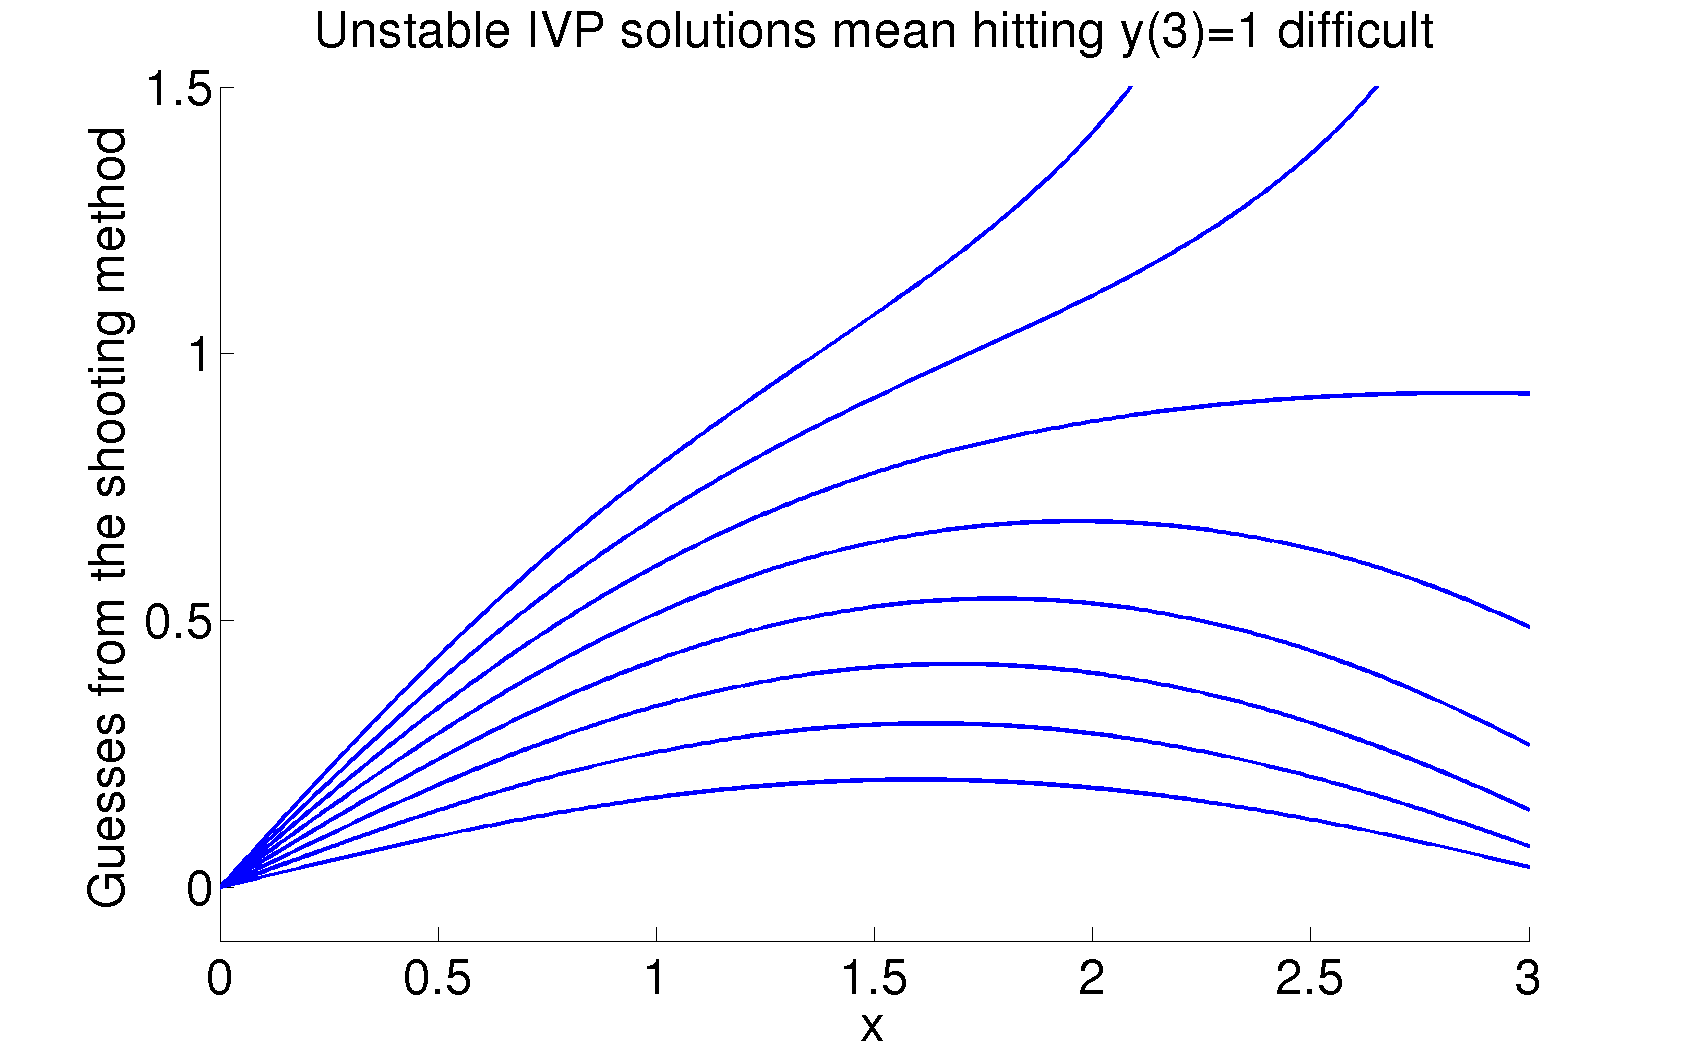
\includegraphics[width=\textwidth]{figures/ShootingProblem3}
      \end{center}
    \end{column}
  \end{columns}
\end{frame}


\section{Summary}

\subsection{Summary}

\begin{frame}
  \frametitle{Summary}

  \begin{itemize}
  \item Boundary value problems (BVPs) are ODEs where not all the
    conditions required to specify the problem on the interval $x \in
    [a,b]$ are given at a single point.
  \item Shooting methods convert the BVP to an IVP with some free
    initial data; the free data is modified to fit the boundary
    conditions at the ``end'' of the interval. This requires nonlinear
    root finding.
  \item The secant method is the standard nonlinear root finding
    method used; if the additional convergence of Newton's method is
    required the variational equation is typically needed to evaluate
    the derivative of the nonlinear function.
  \item Shooting methods, when they work, are fast and
    accurate. However, they fail to \emph{exactly} satisfy the
    boundary conditions at the ``end'' of the interval, and there are
    problems for which the BVP is well-posed but the IVP used in the
    shooting method is not.
  \end{itemize}

\end{frame}

\end{document}



%%% Local Variables:
%%% mode: latex
%%% TeX-master: t
%%% End:
